\section{Auswertung}
\label{sec:Auswertung}

\subsection{Empfindlichkeit der Braunschen Röhre}
Um die Empfindlichkeit $\frac{D}{U_\mathrm{d}}$ zu ermitteln, wird für die sieben Messreihen (siehe Tabelle \ref{tab:messwerte1}) bis \ref{tab:messwerte5} bei unterschiedlichen Beschleunigugsspannungen $U_\mathrm{B}$ jeweils die Auslenkung $D$ gegen die Ablenkspannung $U_\mathrm{d}$ aufgetragen. Mittels einer linearen Ausgleichsrechnung wird die Steigung der Geraden der Form $D(U_d)=a\cdot U_d+b$, welche der Empfindlichkeit entspricht, bestimmt. Dargestellt ist dies in den Abbildungen \ref{fig:empfindlichkeit1} bis \ref{fig:empfindlichkeit7}.

\begin{table}
\centering
  \caption{Messwerte zur Ablenkspannung $U_\mathrm{d}$ und zur Ablenkung $D$ bei verschiedenen Beschleunigungsspannungen $U_\mathrm{B}$.}
  \label{tab:messwerte1}
  \resizebox{\textwidth}{!}{
  \begin{tabular}{c c c c}
    \toprule
    Ablenkung $D/\si{\meter}$ & Ablenkspannung $U_d(U_\mathrm{B}=200\si{\volt})/\si{\volt}$ & Ablenkspannung $U_d(U_\mathrm{B}=250\si{\volt})/\si{\volt}$
    & Ablenkspannung $U_d(U_\mathrm{B}=300\si{\volt})/\si{\volt}$\\
    \midrule
 -0,025 & -20,43 & -25,50 & -30,40 \\
-0,0191 & -16,85 & -21,59 & -25,03\\
 -0,012 & -13,44 & -16,95 & -20,04\\
 -0,006 & -9,64 & -12,29 & -14,72 \\
 0 & -6,15 & -7,76 & -9,19   \\
 0,006 & -2,49 & -3,24 & -3,90  \\
 0,013 & 1,22 & 1,24 & 1,84 \\
 0,019 & 4,98 & 6,19 & 7,92 \\
 0,025 & 7,89 & 10,51 & 13,27  \\
\bottomrule
\end{tabular}
}
\end{table}

\begin{table}
  \caption{Messwerte zur Ablenkspannung $U_\mathrm{d}$ und zur Ablenkung $D$ bei $U_\mathrm{B}=350$.}
  \centering
  \label{tab:messwerte2}
  \begin{tabular}{c c}
    \toprule
   Ablenkung $D/\si{\meter}$ &  Ablenkspannung $U_d/\si{\volt}$\\
    \midrule
-0,024 &-33,96 \\
-0,019 & -29,50 \\
-0,013 & -23,86 \\
-0,006 & -17,05 \\
0 & -10,79 \\
0,006 & -4,46 \\
0,013 & 2,49 \\
0,019 & 8,49 \\
0,025 & 15,36 \\
    \bottomrule
    \end{tabular}
\end{table}

\begin{table}
  \caption{Messwerte zur Ablenkspannung $U_\mathrm{d}$ und zur Ablenkung $D$ bei $U_\mathrm{B}=400$.}
  \centering
  \label{tab:messwerte3}
  \begin{tabular}{c c }
    \toprule
   Ablenkung $D/\si{\meter}$ & Ablenkspannung $U_d/\si{\volt}$\\
    \midrule
-0,021 &-34,60 \\
-0,019 & -32,82 \\
-0,013 & -26,18 \\
-0,006 & -19,28 \\
0 & -12,26 \\
0,006 & -5,24 \\
0,013 & 2,15 \\
0,019 & 9,66 \\
0,025 & 16,76 \\
    \bottomrule
    \end{tabular}
\end{table}

\begin{table}
  \caption{Messwerte zur Ablenkspannung $U_\mathrm{d}$ und zur Ablenkung $D$ bei $U_\mathrm{B}=450$.}
  \centering
  \label{tab:messwerte4}
  \begin{tabular}{c c }
    \toprule
    Ablenkung $D/\si{\meter}$ &  Ablenkspannung $U_d/\si{\volt}$\\
    \midrule
-0,016 &-33,85 \\
-0,014 & -31,38 \\
-0,013 & -26,69 \\
-0,006 & -21,80 \\
0 & -13,89 \\
0,006 & -5,87 \\
0,013 & 2,32 \\
0,019 & 10,37 \\
0,025 & 18,93 \\
    \bottomrule
    \end{tabular}
\end{table}

\begin{table}
  \caption{Messwerte zur Ablenkspannung $U_\mathrm{d}$ und zur Ablenkung $D$ bei $U_\mathrm{B}=500$.}
  \centering
  \label{tab:messwerte5}
  \begin{tabular}{c c }
    \toprule
    Ablenkung $D/\si{\meter}$ &    Ablenkspannung $U_d/\si{\volt}$\\
    \midrule
-0,014 &-34,52 \\
-0,013 & -32,93 \\
-0,010 & -28,12 \\
-0,006 & -23,72 \\
0 & -15,33 \\
0,006 & -6,46 \\
0,013 & 2,57\\
0,019 & 12,02 \\
0,025 & 21,21 \\
    \bottomrule
    \end{tabular}
\end{table}

\begin{figure}
  \centering
  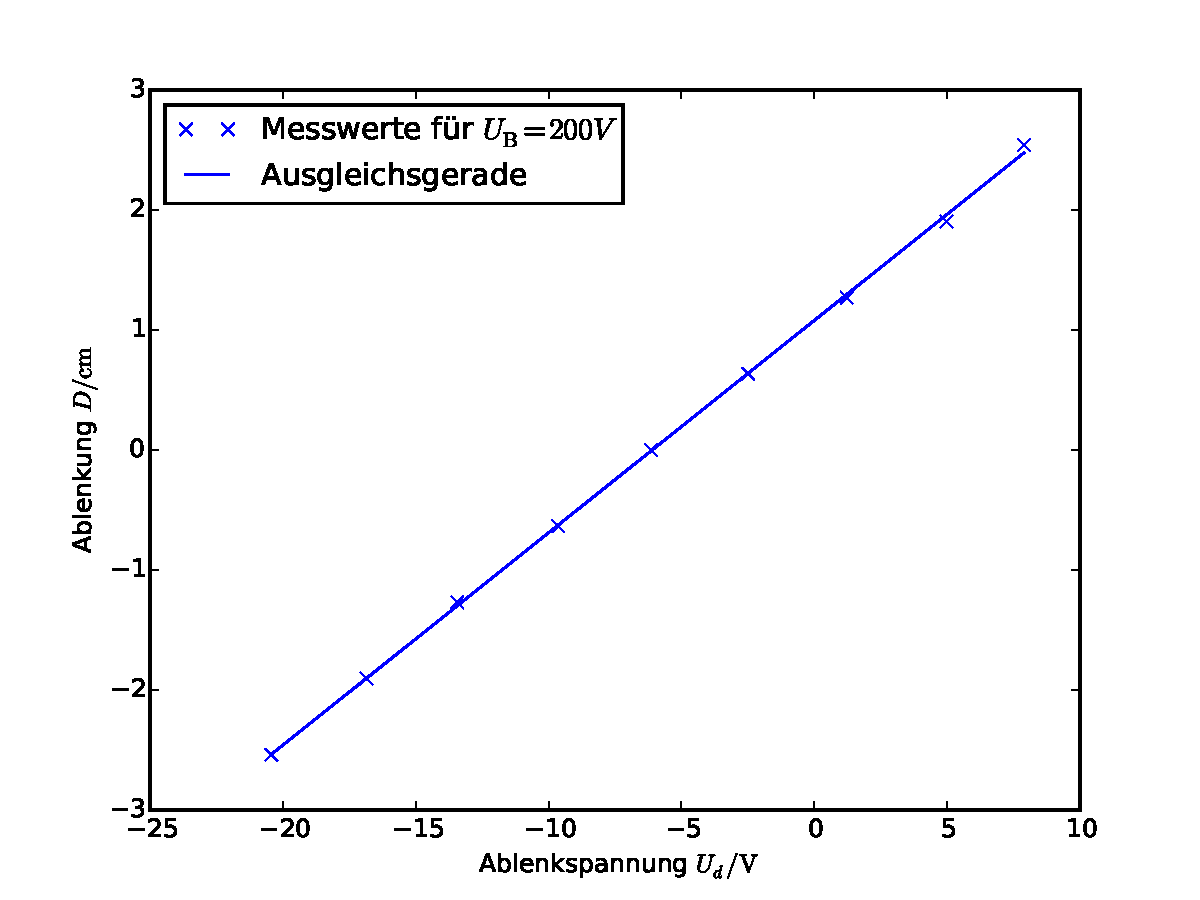
\includegraphics[scale=0.8]{auswertung/501-a1.pdf}
\caption{Ablenkung $D$ in Abhängigkeit von $U_\mathrm{d}$ für $U_\mathrm{B}$ 200 \si{\volt}.}
  \label{fig:empfindlichkeit1}
\end{figure}

\begin{figure}
  \centering
  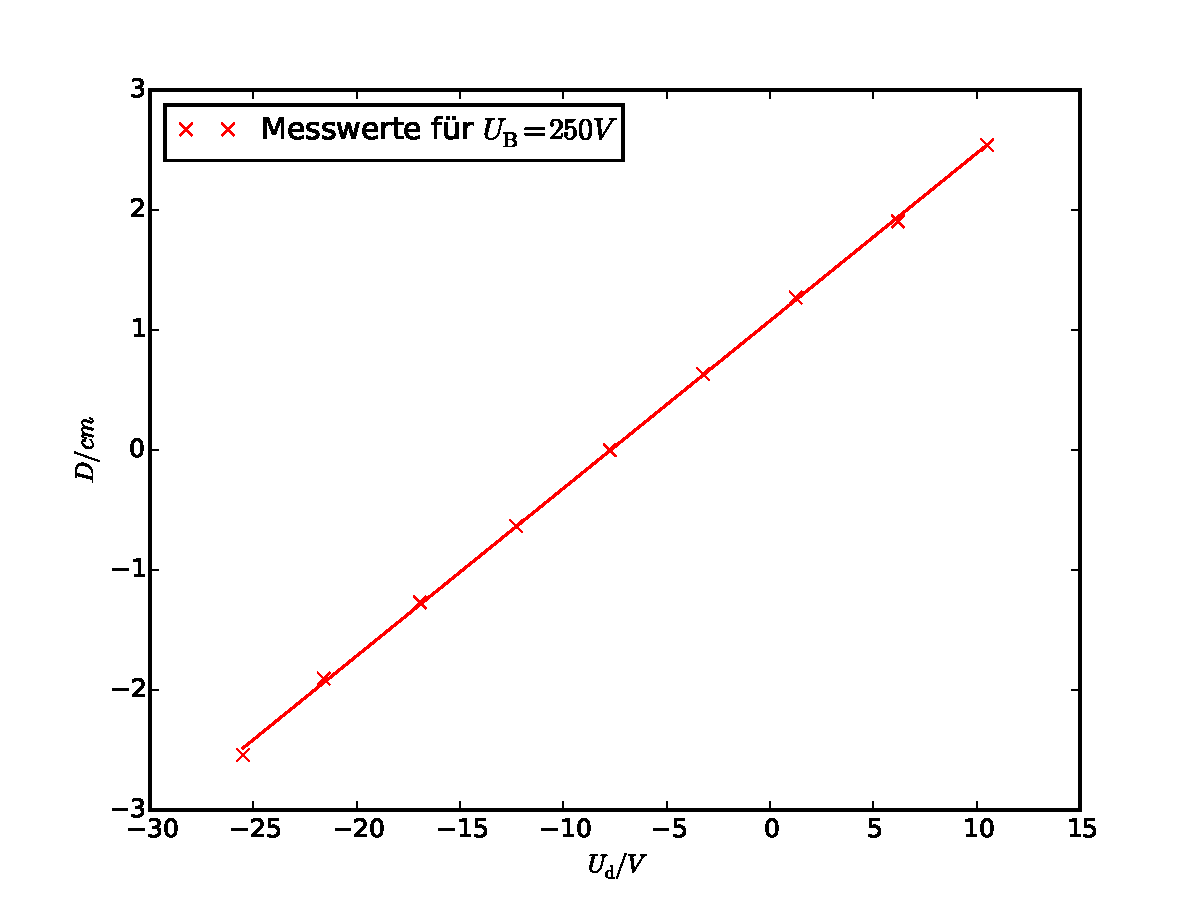
\includegraphics[scale=0.8]{auswertung/501-a-2.pdf}
\caption{Ablenkung $D$ in Abhängigkeit von $U_\mathrm{d}$ für $U_\mathrm{B}$ 250\si{\volt}.}
  \label{fig:empfindlichkeit2}
\end{figure}

\begin{figure}
  \centering
  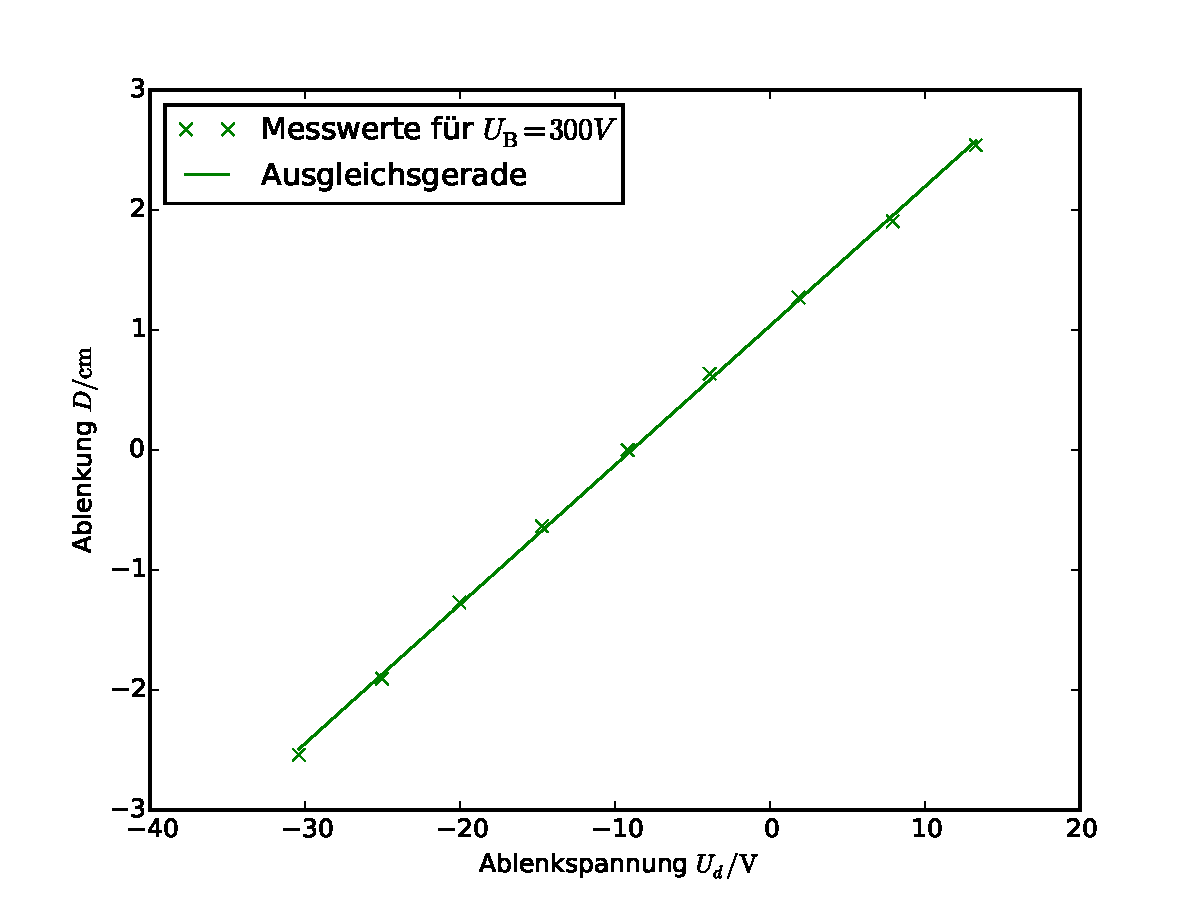
\includegraphics[scale=0.8]{auswertung/501-a-3.pdf}
\caption{Ablenkung $D$ in Abhängigkeit von $U_\mathrm{d}$ für $U_\mathrm{B}$ 300\si{\volt}.}
  \label{fig:empfindlichkeit3}
\end{figure}

\begin{figure}
  \centering
  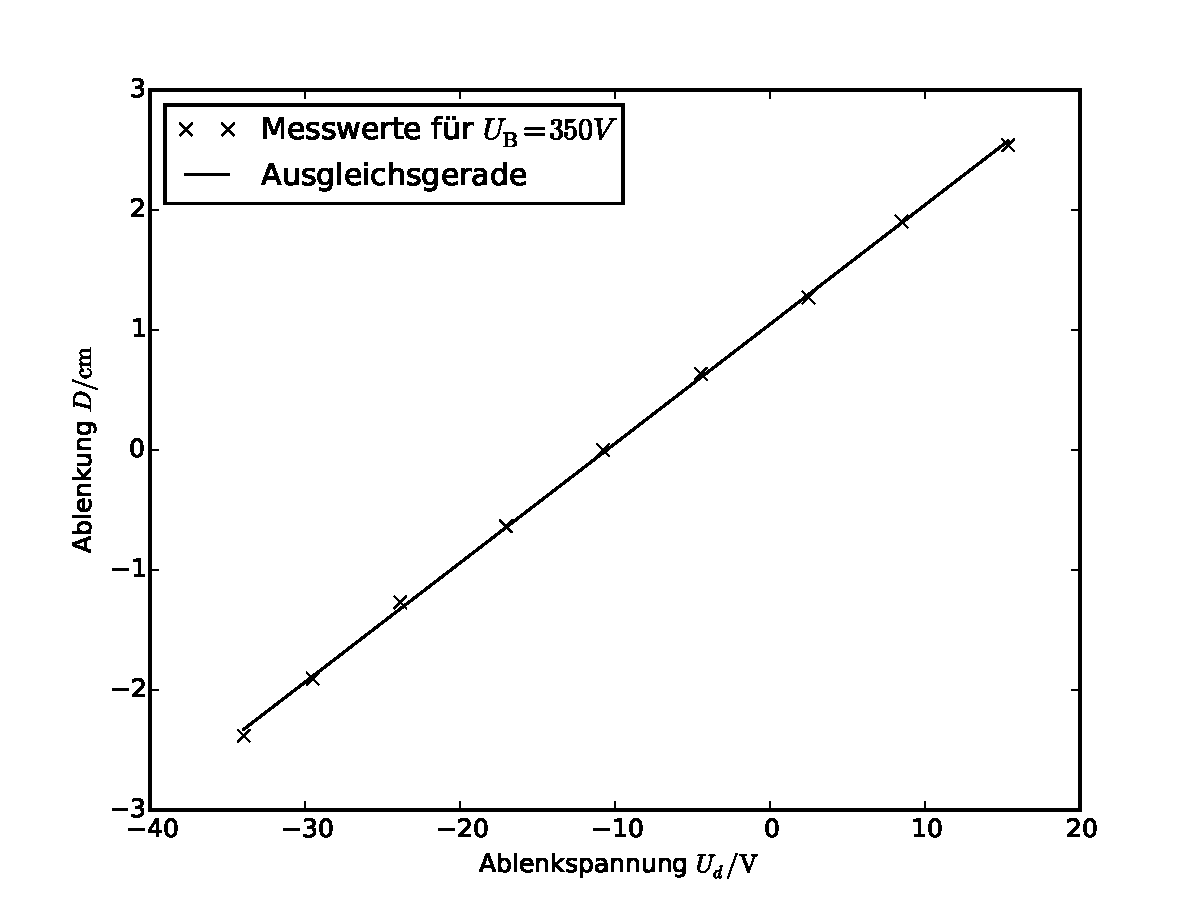
\includegraphics[scale=0.8]{auswertung/501-a4.pdf}
\caption{Ablenkung $D$ in Abhängigkeit von $U_\mathrm{d}$ für $U_\mathrm{B}$ 350\si{\volt}.}
  \label{fig:empfindlichkeit4}
\end{figure}

\begin{figure}
  \centering
  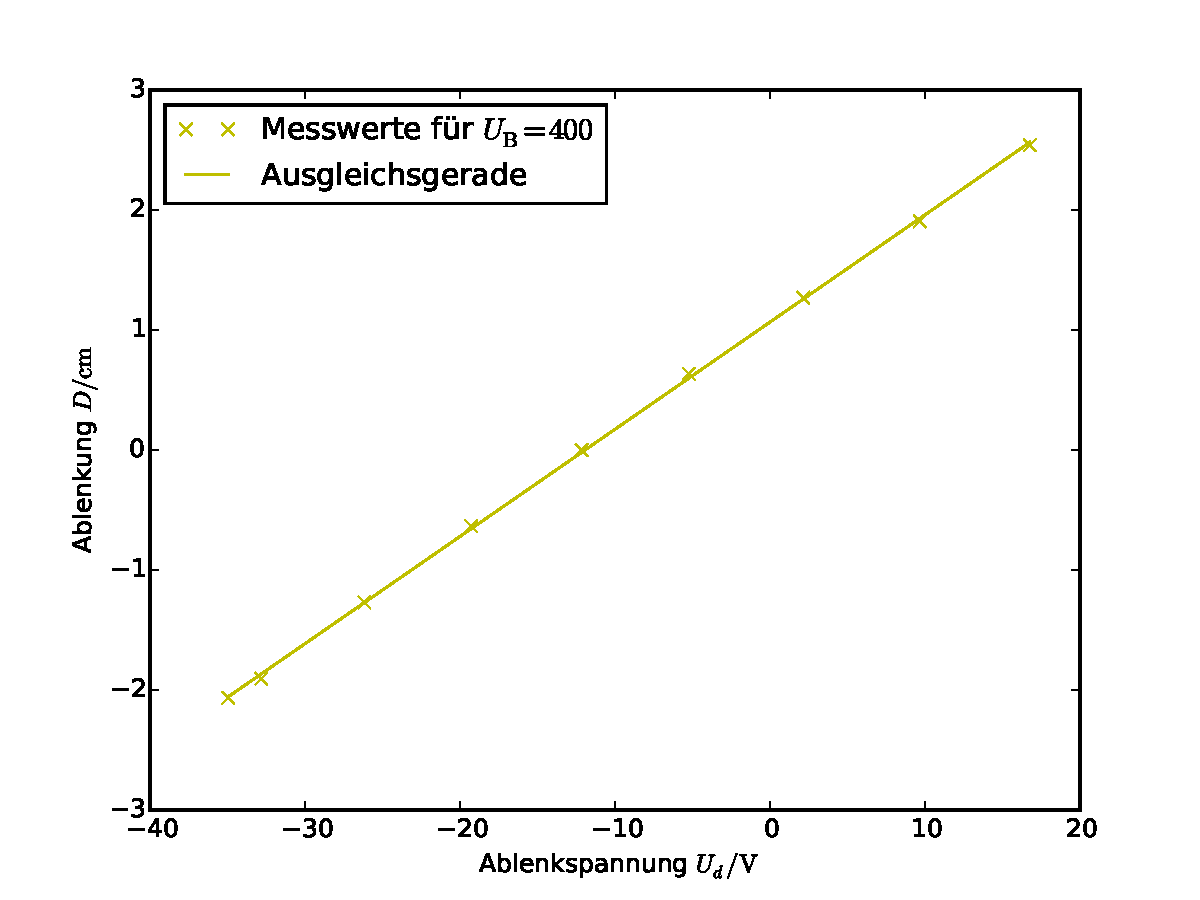
\includegraphics[scale=0.8]{auswertung/501-a5.pdf}
\caption{Ablenkung $D$ in Abhängigkeit von $U_\mathrm{d}$ für $U_\mathrm{B}$ 400\si{\volt}.}
  \label{fig:empfindlichkeit5}
\end{figure}

\begin{figure}
  \centering
  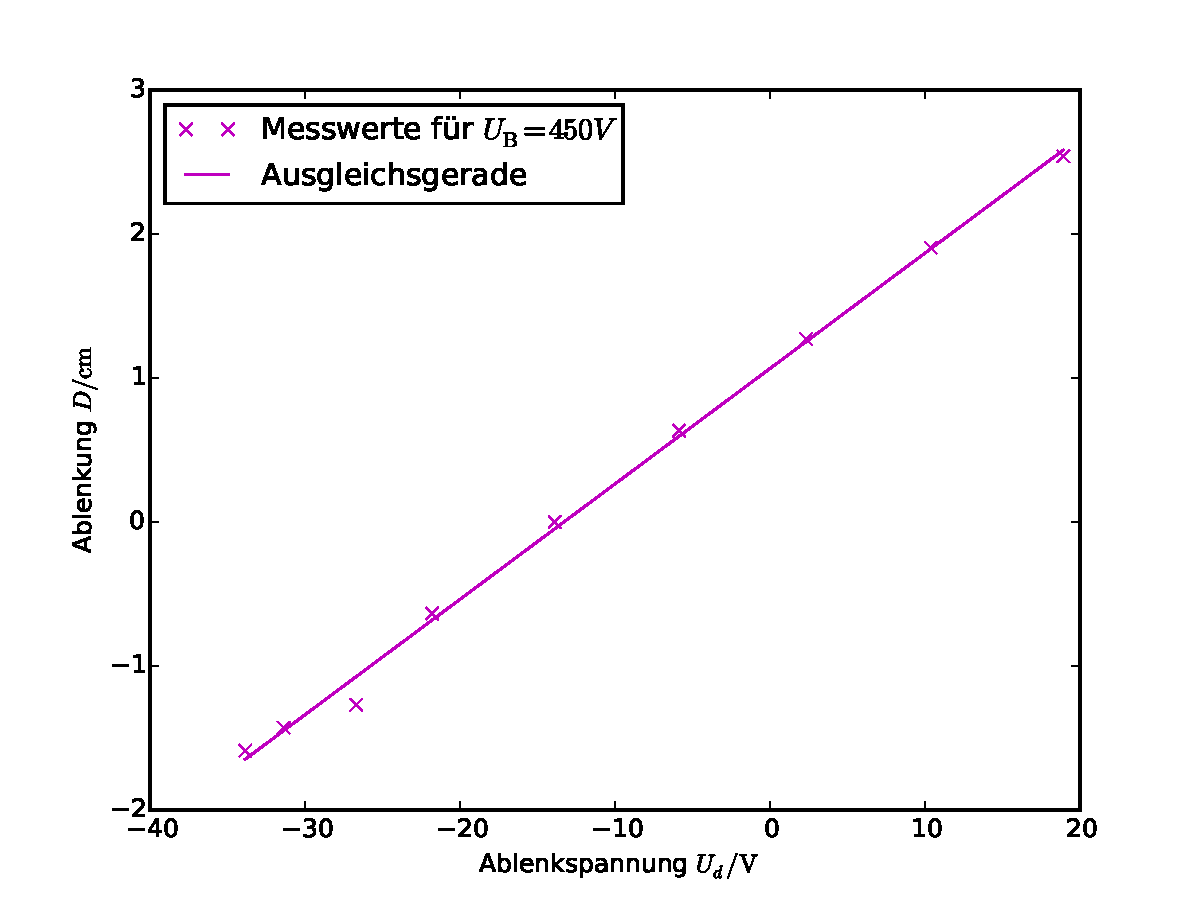
\includegraphics[scale=0.8]{auswertung/501-a6.pdf}
\caption{Ablenkung $D$ in Abhängigkeit von $U_\mathrm{d}$ für $U_\mathrm{B}$ 450\si{\volt}.}
  \label{fig:empfindlichkeit6}
\end{figure}

\begin{figure}
  \centering
  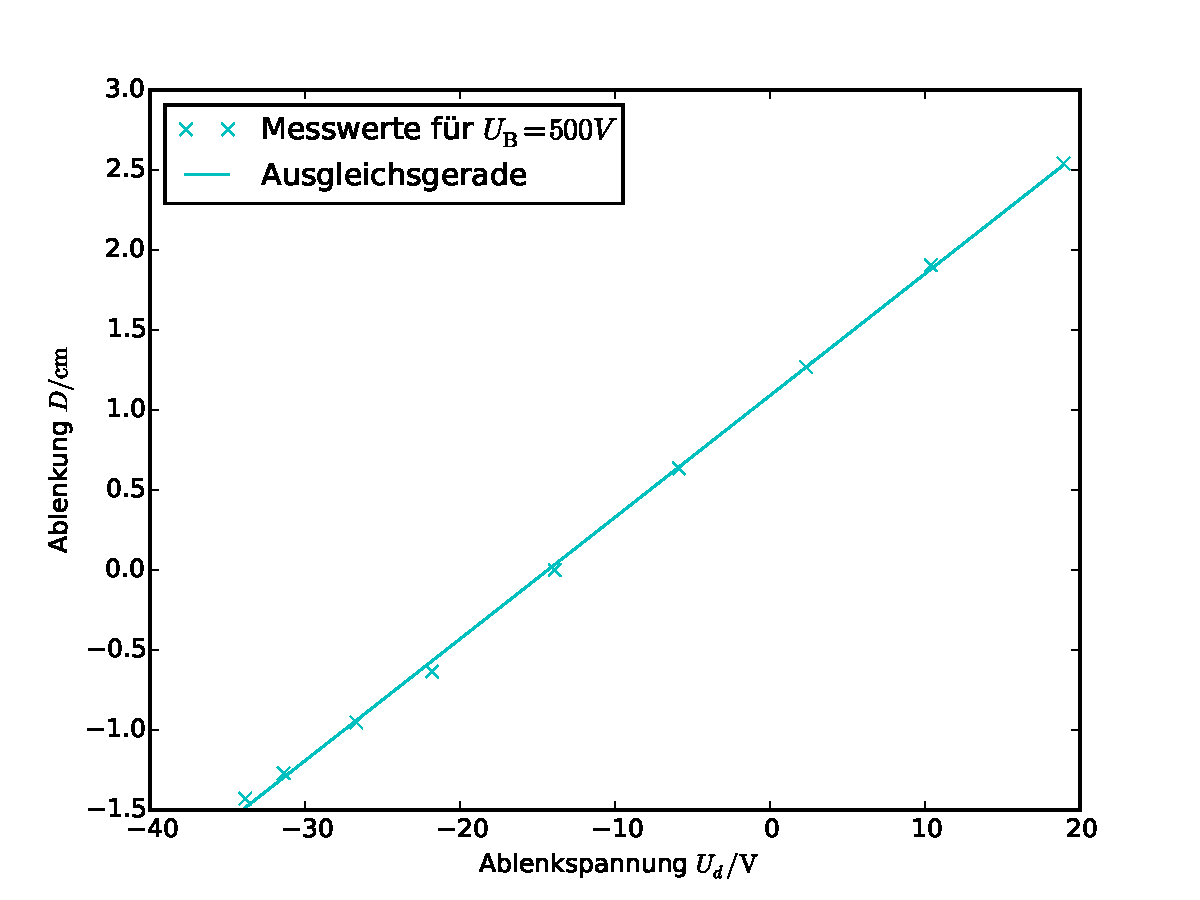
\includegraphics[scale=0.8]{auswertung/501-a7.pdf}
\caption{Ablenkung $D$ in Abhängigkeit von $U_\mathrm{d}$ für $U_\mathrm{B}$ 500\si{\volt}.}
  \label{fig:empfindlichkeit7}
\end{figure}


Die berechneten Werte für Die Steigung und den y-Achsenabschnitt der Geraden befinden sich in Tabelle \ref{tab:empfindlichkeit}.

\begin{table}
  \caption{Werte für die Steigungen der Ausgleichsgeraden.}
  \centering
  \label{tab:empfindlichkeit}
  \begin{tabular}{c c c}
    \toprule
     Beschleunigungsspannung $U_\mathrm{B} / \si{\volt}$ &  Empfindlichkeit $\frac{D}{U_\mathrm{d}}/ 10^{-2} \frac{\si{\meter}}{\si{\volt}}$ & $b / 10^{-2}\si{\meter}$ \\
    \midrule
200 & 0,177 \pm 0,001 & 1,078 \pm 0,014 \\
250 & 0,140 \pm 0,001 & 1,077 \pm 0,012 \\
300 & 0,116 \pm 0,001 & 1,035 \pm 0,017 \\
350 & 0,099 \pm 0,001 & 1,048 \pm 0,015 \\
400 & 0,089 \pm 0,001 & 1,066 \pm 0,011 \\
450 & 0,080 \pm 0,002 & 1,066 \pm 0,034 \\
500 & 0,076 \pm 0,001 & 1,090 \pm 0,015 \\
\bottomrule
\end{tabular}
\end{table}

Damit ergibt sich für die Empfindlichkeit gemittelt $\langle\frac{D}{U_\mathrm{d}}\rangle=(0.0100 \pm 0.0004)10^{-2}\frac{\si{\meter}}{\si{\volt}}$.

\subsection{Bestimmung der Apparaturkonstante}
Die zuvor bestimmten Empfindlichkeiten sollen nun gegen $\frac{1}{U_\mathrm{B}}$ aufgetragen werden(siehe Abbildung \ref{fig:A}). erneut wird mittels linearer Ausgleichrechung die Steigung bestimmt und soll mit der Konstante $A=\frac{pL}{2d}$ verglichen werden.

\begin{figure}
  \centering
  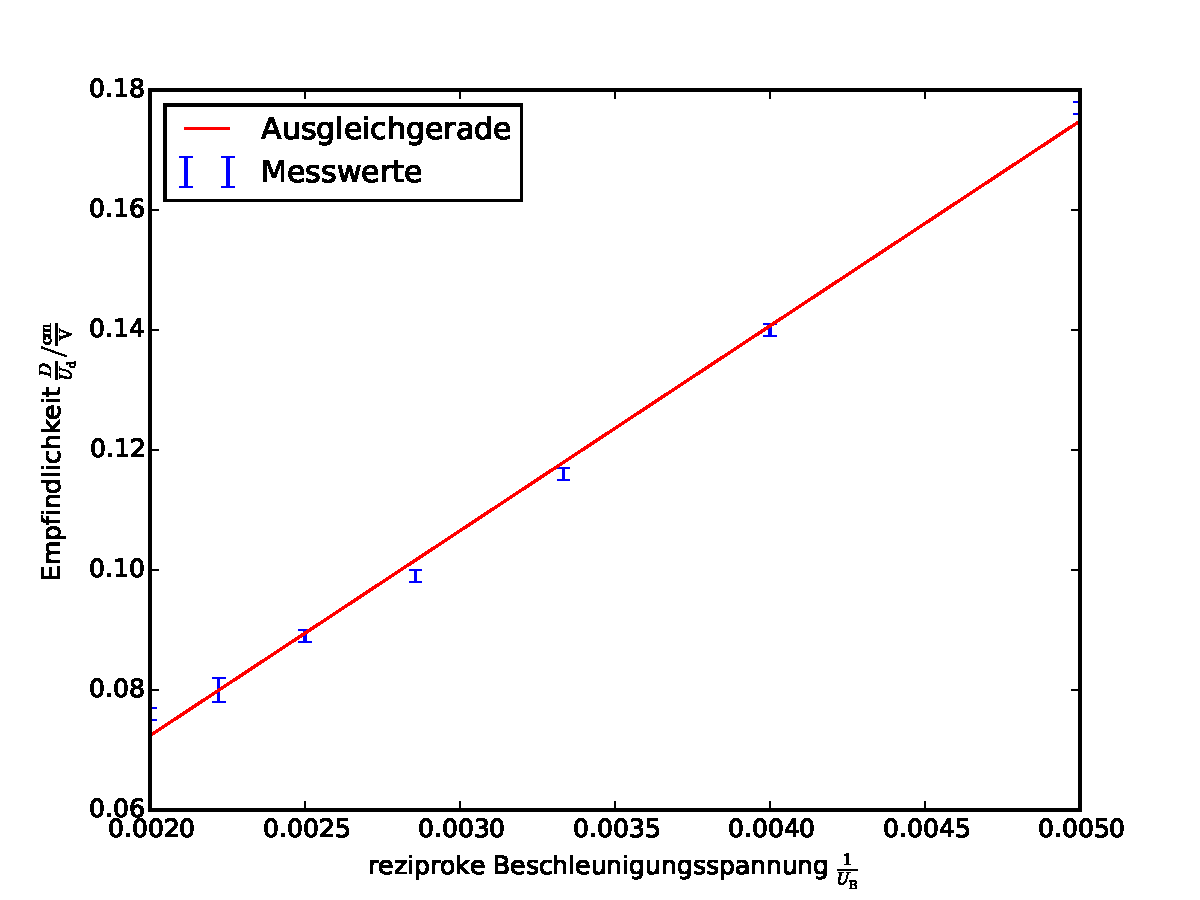
\includegraphics[scale=0.8]{auswertung/501-a3.pdf}
\caption{ Empfindlichkeit $\frac{D}{U_\mathrm{d}}$ in Abhängigkeit von der reziproken Beschleunigungsspannung $\frac{1}{U_\mathrm{B}}$ .}
  \label{fig:A}
\end{figure}

Für die Gerade gilt erneut $D(U_d)=a\cdot U_d+b$. Für $a$ und $b$ ergeben sich folgende Werte:
\begin{align}
  a&=(34,147 \pm 0,972)10^{-2}\si{\meter}\\
  b&=(0,004 \pm 0,003)\frac{10^{-2}\si{\meter}}{\si{\volt}}\\
\end{align}
Mit
\begin{align}
  p&=0,0019 \si{\meter}\\
  l&=0,1533 \si{\meter} \\
  d&=0,000665 \si{\meter}\\
\end{align}
ergibt sich für $A=0,438$ \si{\meter}. Das entspricht einer Abweichung von $(28 \pm 0,04)\%$ zur berechneten Steigung der Ausgleichsgeraden.

\subsection{Kathodenstrahl-Oszillograph}
Im folgenden Teil soll aus den vier gemessenen Frequenzen der Sägezahnspannung die Frequenz der anliegenden Sinusspannung ermittelt sowie ih Scheitelwert berechnet werden. Die gemessenen Frequenzen befinden sich in Tabelle \ref{tab:frequenzen}.

\begin{table}
  \caption{Werte für die Steigungen der Ausgleichsgeraden.}
  \centering
  \label{tab:frequenzen}
  \begin{tabular}{c c c}
    \toprule
    $f / \si{\Hz}$ & $D/\si{\meter}$ &$n$ \\
    \midrule
79,87 & 0,01905 & 1 \\
39,95 & 0,01905 & 2\\
159,75 & 0,01905 & 1/2\\
239,37 & 0,01905 & 1/3\\
\bottomrule
\end{tabular}
\end{table}

Mit der Synchronisationsbedingung $n f_\mathrm{Sä}= m f_\mathrm{sin}$ folgt, dass $f_\mathrm{sin}=79,87$ \si{\Hz}.
Setzt man die Empfindlichkeit mit $\frac{D}{U_\mathrm{sin}}$ gleich, erhält man.
\begin{equation}
  (0.0100 \pm 0.0004)10^{-2}\frac{\si{\meter}}{\si{\volt}} = \frac{0,01905 \si{\meter}}{U_\mathrm{sin}}
\Rightarrow U_\mathrm{sin} = 19,5 \si{\volt}.
\end{equation}

\subsection{Ablenkung der Elektronen im Magnetfeld}
Die gemessenen Spulenströme für verschiedene Beschleunigungsspannungen sind in Tabelle \ref{tab:messwerte-a} bis \ref{tab:messwerte-e} dargestellt. Das $B$-Feld innerhalb der Spule kann mit Formel \eqref{eqn:spule} berechnet werden. Nun soll, wie in Abbildung \ref{fig:spez.ladung1} und \ref{fig:spez.ladung2} dargestellt, $\frac{D}{L^2+D^2}$ gegen $B$ aufgetragen werden und aus der Steigung der Ausgleichsgeraden die spezifische Ladung $\frac{e}{m_\mathrm{e}}$ bestimmt werden.


\begin{table}
  \caption{Messwerte zur Ablenkung $D$, zum Spulenstrom $I_\mathrm{S}$ und dem daraus resultierenden $B$-feld bei der Beschleunigungsspannung $U_\mathrm{B}=250 \si{\volt}$.}
  \centering
  \label{tab:messwerte-a}
  \begin{tabular}{c c c}
    \toprule
      Ablenkung $D/\si{\meter}$ & $I_\mathrm{s}/\si{\ampere}$ & $B$/\si{\milli\tesla}\\
    \midrule
 0 & 0 & 0\\
0,0254 & 0,27 & 0,017 \\
0,0508 & 0,60  & 0,038\\
0,0762 & 0,91  & 0,058\\
0,1016 & 1,25  & 0,080\\
0,127 & 1,58  & 0.101\\
0,1524 & 1,91 & 0,122\\
0,1778 & 2,25  & 0,143\\
0,2032 & 2,59  & 0,165\\
\bottomrule
\end{tabular}
\end{table}

\begin{table}
  \caption{Messwerte zur Ablenkung $D$, zum Spulenstrom $I_\mathrm{S}$ und dem daraus resultierenden $B$-feld bei der Beschleunigungsspannung $U_\mathrm{B}=300 \si{\volt}$.}
  \centering
  \label{tab:messwerte-b}
  \begin{tabular}{c c c}
    \toprule
      Ablenkung $D/\si{\meter}$ & $I_\mathrm{s}/\si{\ampere}$ & $B$/\si{\milli\tesla}\\
    \midrule
0  & 0 &0\\
0,0254 &0,32 & 0,20 \\
0,0508 & 0,67 & 0,043 \\
0,0762 & 1,04  & 0,066\\
0,1016 & 1,38  & 0,088\\
0,127 & 1,75  & 0,112\\
0,1524 & 2,09  & 0,133\\
0,1778 & 2,45  & 0,156\\
0,2032 & 2,81  & 0,179\\
\bottomrule
\end{tabular}
\end{table}

\begin{table}
  \caption{Messwerte zur Ablenkung $D$, zum Spulenstrom $I_\mathrm{S}$ und dem daraus resultierenden $B$-feld bei der Beschleunigungsspannung $U_\mathrm{B}=350 \si{\volt}$.}
  \centering
  \label{tab:messwerte-c}
  \begin{tabular}{c c c}
    \toprule
      Ablenkung $D/\si{\meter}$ & $I_\mathrm{s}/\si{\ampere}$ & $B$/\si{\milli\tesla}\\
    \midrule
0  & 0 & 0\\
0,0254 & 0,33 & 0,021 \\
0,0508 & 0,70 & 0,045\\
0,0762 & 1,09 & 0,070 \\
0,1016 & 1,47  & 0,094\\
0,127 & 1,84  & 0,117\\
0,1524 & 2,27 & 0,145 \\
0,1778 &2,68  & 0,171\\
0,2032 & 3,02 & 0,193 \\
\bottomrule
\end{tabular}
\end{table}

\begin{table}
  \caption{Messwerte zur Ablenkung $D$, zum Spulenstrom $I_\mathrm{S}$ und dem daraus resultierenden $B$-feld bei der Beschleunigungsspannung $U_\mathrm{B}=400 \si{\volt}$.}
  \centering
  \label{tab:messwerte-d}
  \begin{tabular}{c c c}
    \toprule
      Ablenkung $D/\si{\meter}$ & $I_\mathrm{s}/\si{\ampere}$ & $B$/\si{\milli\tesla}\\
    \midrule
0  & 0 &  0\\
0,0254 & 0,4 & 0,026\\
0,0508 & 0,77 & 0,049\\
0,0762 & 1,22 & 0,078 \\
0,1016 & 1,63  & 0,104\\
0,127 & 2,05 & 0,131\\
0,1524 & 2,49 & 0,159 \\
0,1778 & 2,88  0,184\\
0,2032 & / & /\\
\bottomrule
\end{tabular}
\end{table}

\begin{table}
  \caption{Messwerte zur Ablenkung $D$, zum Spulenstrom $I_\mathrm{S}$ und dem daraus resultierenden $B$-feld bei der Beschleunigungsspannung $U_\mathrm{B}=450 \si{\volt}$.}
  \centering
  \label{tab:messwerte-e}
  \begin{tabular}{c c c}
    \toprule
      Ablenkung $D/\si{\meter}$ & $I_\mathrm{s}/\si{\ampere}$ & $B$/\si{\milli\tesla}\\
    \midrule
0  & 0 & 0 \\
0,0254 & 0,41 & 0,026 \\
0,0508 & 0,82 & 0,052\\
0,0762 & 1,28 & 0,082\\
0,1016 & 1,69 & 0,108 \\
0,127 & 2,12 & 0,135\\
0,1524 & 2,58 & 0,165\\
0,1778 & 3,01  0,192\\
0,2032 & / & / \\
\bottomrule
\end{tabular}
\end{table}

\begin{figure}
  \centering
  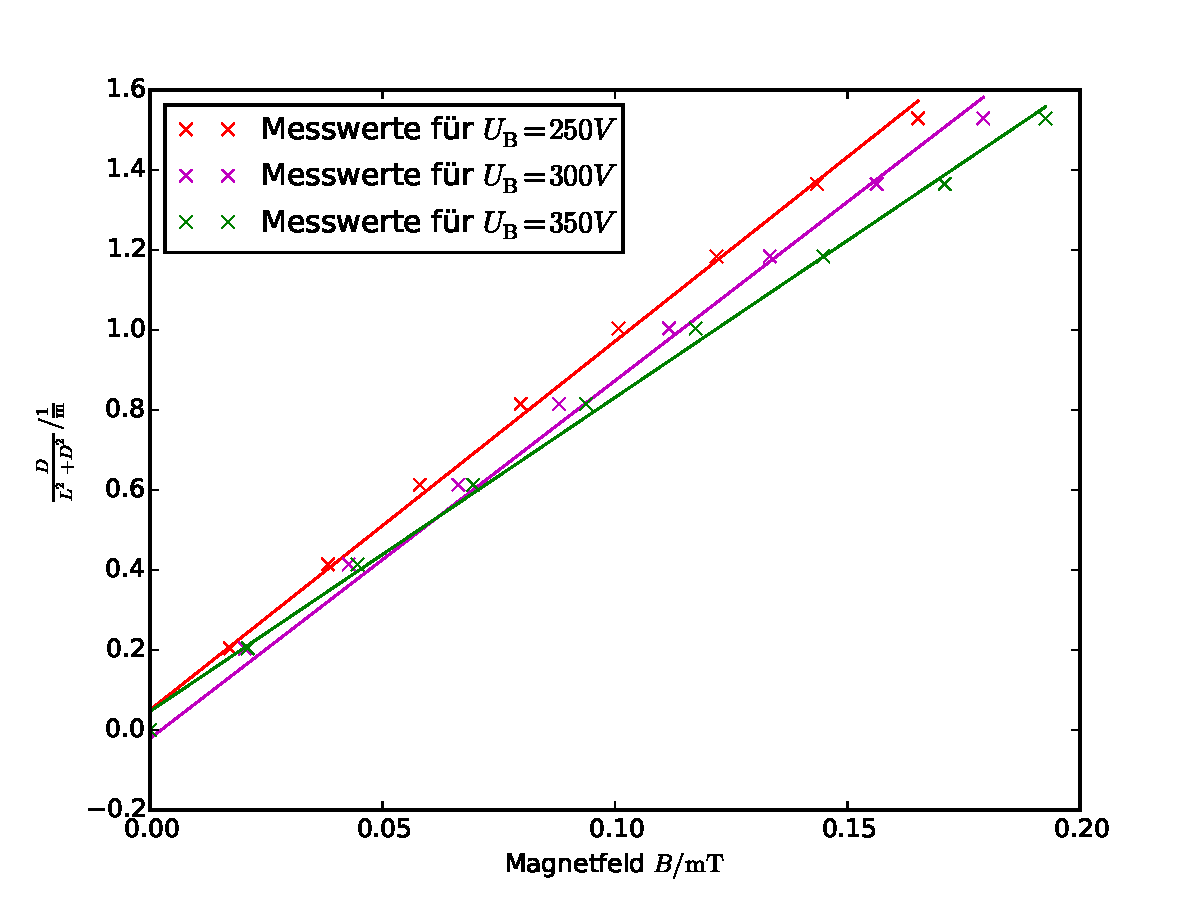
\includegraphics[scale=0.8]{auswertung/502-a.pdf}
\caption{$\frac{D}{L^2+D^2}$ in Abhängigkeit von $B$ für $U_\mathrm{B} 250 - 350 \si{\volt}$.}
  \label{fig:spez.ladung1}
\end{figure}

\begin{figure}
  \centering
  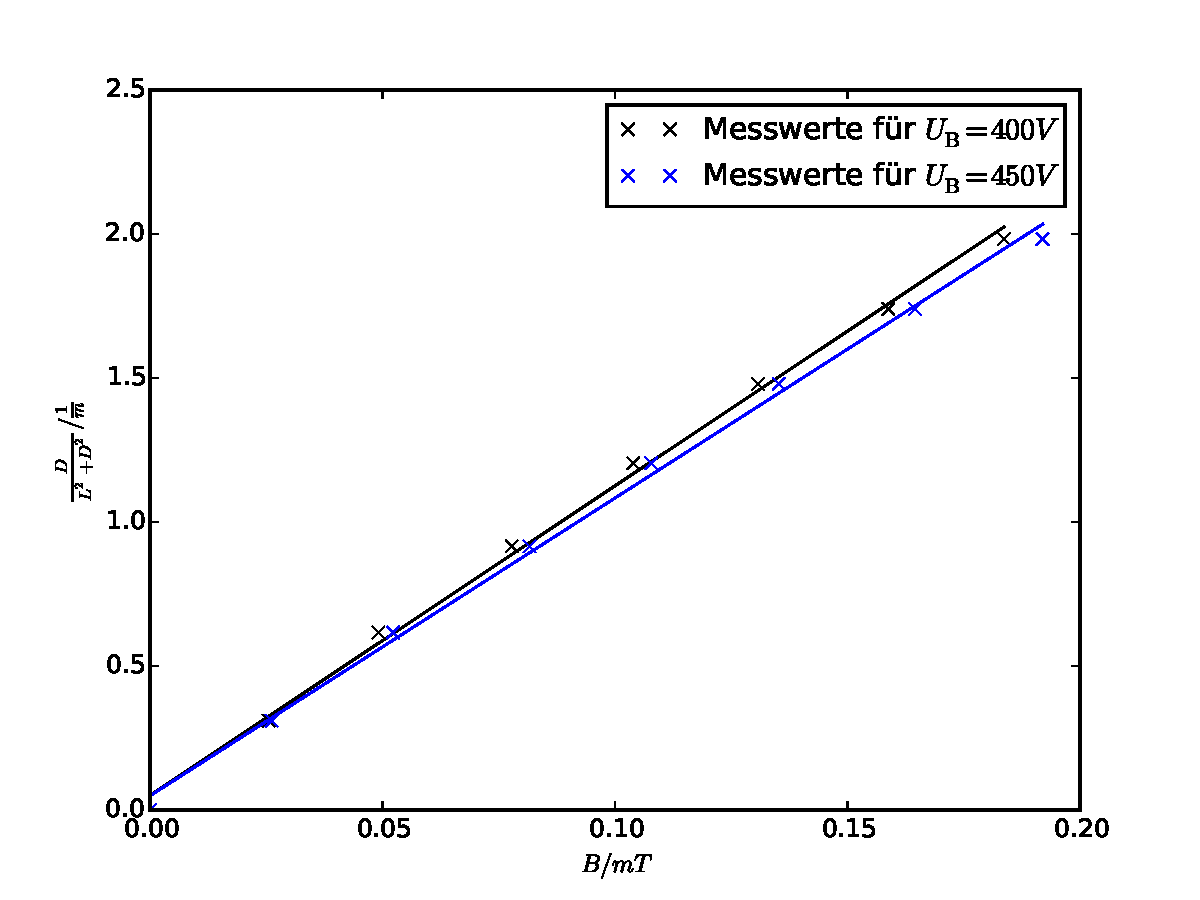
\includegraphics[scale=0.8]{auswertung/502-a2.pdf}
\caption{$\frac{D}{L^2+D^2}$ in Abhängigkeit von $B$ für $U_\mathrm{B} 400 - 500 \si{\volt}$.}
  \label{fig:spez.ladung2}
\end{figure}

Für alle geraden gilt $y=ax+b$. Die Werte der Parameter für die Ausgleichsgeraden befinden sich in Tabelle \ref{tab:spez.ladung}.
Mit Gleichung \eqref{eqn:spez} folgt für die spezifische Ladung
\begin{equation}
  \frac{e}{m_\mathrm{e}}=8U_\mathrm{B}a^2.
\end{equation}
Die Werte hierzu befinden sich ebenfalls in \ref{tab:spez.ladung}.

\begin{table}
  \caption{Werte für die Steigungen der Ausgleichsgeraden und die daraus ermittelte spezifische Ladung.}
  \centering
  \label{tab:spez.ladung}
  \begin{tabular}{c c c c}
    \toprule
     $U_\mathrm{B} / \si{\volt}$ & $a/ \frac{1}{\si{\meter\milli\tesla}}$ & $b / \frac{1}{\si{\meter}}$ & $\frac{e}{m_\mathrm{e}}/\frac{\si{\coulomb}}{\si{\kilo\gram}}10^11$ \\
    \midrule
250 & 9,218 \pm 0,197 & 0,050 \pm 0,019 & 1,70 \pm 0,07  \\
300 & 8,945 \pm 0,040 & -0,021 \pm 0,019 & 1,92 \pm 0,16 \\
350 & 7,849 \pm 0,162 & 0,046 \pm 0,019 & 1,72 \pm 0,07\\
400 & 7,389 \pm 0,121 & 0,026 \pm 0,013 & 1,75 \pm 0,06\\
450 & 7,110 \pm 0,115 & 0,024 \pm 0,013 & 1,82 \pm 0,06\\
\bottomrule
\end{tabular}
\end{table}

Damit ergibt sich für die spezifische Ladung ein Mittelwert von $\langle\frac{e}{m_\mathrm{e}}\rangle=(1,78 \pm 0,04)10^11 \frac{\si{\coulomb}}{\si{\kilo\gram}}$.

\subsection{Bestimmung der Totalintensität des Erdmagnetfeldes}
Für den Spulestrom und dem Inklinationswinkel werden folgende Werte gemessen:
\begin{align}
  I_\mathrm{hor}&=0,12 \si{\ampere}\\
  \phi &= 72,5^\circ \\
\end{align}

Es wird erneut Gleichung \eqref{eqn:spule} für das $B$-Feld innerhalb einer Helmholtzspule verwendet. Mit der gemessenen Stromstärke ergibt sich die Horizontalkomponente des Erdmagnetfeldes. Für die Totalintensität gilt
\begin{equation}
  B_\mathrm{total}=\frac{B_\mathrm{hor}}{\cos(\phi)}.
\end{equation}
Damit ergibt sich $B_\mathrm{total}=2,54 \cdot 10^{-5}\si{\tesla}$.
